%%%%%%%%%%%%%%%%%%%%%%%%%%%%%%%%%%%%%%%%%%%%%%%%%%%%
% Document type, global settings, and packages
%%%%%%%%%%%%%%%%%%%%%%%%%%%%%%%%%%%%%%%%%%%%%%%%%%%%

\documentclass[12pt]{report}
\usepackage{graphicx}
\usepackage[letterpaper, margin=1in]{geometry}
\usepackage{setspace}  % use this package to set line spacing as desired
\usepackage{times}  % set Times New Roman as the font
\usepackage[explicit]{titlesec}  % title control and formatting
\usepackage[titles]{tocloft}  % table of contents control and formatting
\usepackage{inputenc}
\usepackage[backend=biber, bibstyle=ieee]{biblatex}
\usepackage[bookmarks=true, hidelinks]{hyperref}
% \usepackage[page]{appendix}  % for appendices
% \usepackage{rotating}  % for rotated, landscape images
\usepackage[normalem]{ulem}  % for italicized text
\usepackage{amsmath}
\usepackage{xcolor}
\usepackage{cleveref}
\usepackage{hyperref}


\DeclareUnicodeCharacter{262F}{YIN YANG HERE!!!!!}

%%%%%%%%%%%%%%%%%%%%%%%%%%%%%%%%%%%
% Bibliography settings
%%%%%%%%%%%%%%%%%%%%%%%%%%%%%%%%%%%

% Your bibliography file here
\bibliography{references.bib}

% prevent certain fields in references from printing in the bibliography
\AtEveryBibitem{\clearfield{issn}}
\AtEveryBibitem{\clearlist{issn}}

\AtEveryBibitem{\clearfield{language}}
\AtEveryBibitem{\clearlist{language}}

\AtEveryBibitem{\clearfield{doi}}
\AtEveryBibitem{\clearlist{doi}}

\AtEveryBibitem{\clearfield{url}}
\AtEveryBibitem{\clearlist{url}}

\AtEveryBibitem{%
  \ifentrytype{online}
    {}
    {\clearfield{urlyear}\clearfield{urlmonth}\clearfield{urlday}}}

%%%%%%%%%%%%%%%%%%%%%%
% Start of Document
%%%%%%%%%%%%%%%%%%%%%%

\begin{document}
\singlespacing %set line spacing

%%%%%%%%%%%%%%%%%%%%%%%%%%%%%%%%%%%%%
% Title Page
%%%%%%%%%%%%%%%%%%%%%%%%%%%%%%%%%%%%%

%% Define your thesis title, name, school, month and year, etc.
\newcommand{\thesisTitle}{Advancing Defensive Magics Against Dark Forces}
\newcommand{\yourName}{Harry Potter}
\newcommand{\yourDept}{Department of Magical Science and Engineering}
\newcommand{\yourSchool}{Hogwarts School of Witchcraft and Wizardry}
\newcommand{\monthYear}{June 2008}
\newcommand{\advisor}{Prof.~Albus Dumbledore}
\newcommand{\committee}{Profs.~Minerva McGonagall, Severus Snape}


%%%%%%%%%%%%%%%%%%%%%%%%%%%%%%%%%%%%%%%%%%%%%%%%%%%%%%%%%
% Do not edit these lines unless you wish to customize
% the template
%%%%%%%%%%%%%%%%%%%%%%%%%%%%%%%%%%%%%%%%%%%%%%%%%%%%%%%%%


\begin{titlepage}
\begin{center}

\begin{doublespacing}
\Large
\vspace{15\baselineskip}
Ph.D.~Dissertation Proposal\\
\vspace{3\baselineskip}

\textbf{\LARGE{Top down and bottom up determinants of ecosystem functioning
}}\\

\vspace{2\baselineskip}
By\\
Michael P. Mustri\\
Advisors: Drs. Scott Saleska and Brian Enquist \\
Committee: Drs. Christopher Kempes and Malak Tfaily\\
\vspace{3\baselineskip}
\large
Ecology and Evolutionary Biology\\
University of Arizona\\
August, 2025

\vfill


\end{doublespacing}

\end{center}
\end{titlepage}

\currentpdfbookmark{Title Page}{titlePage}  %add PDF bookmark for this page

\pagenumbering{roman}
\setcounter{page}{1} % set the page number appropriately

%%%%%%%%%%%%%%%%%%%%%%%%%%%%%%%%%%%%%%%%%%%%%%%%%%%%%%%%%%%%%%%%%
% Abstract if needed
%%%%%%%%%%%%%%%%%%%%%%%%%%%%%%%%%%%%%%%%%%%%%%%%%%%%%%%%%%%%%%%%%
% \input{abstract.tex}

%%%%%%%%%%%%%%%%%%%%%%%%%%%%%%%%%%%%%
% Abbreviations, glossary, nomenclature if needed
%%%%%%%%%%%%%%%%%%%%%%%%%%%%%%%%%%%%%
% \input{abbreviations.tex}
% \input{glossary.tex}
% \input{nomenclature.tex}


%%%%%%%%%%%%%%%%%%%%%%%%%%%%%%%%%%%%%
% Table of Contents
%%%%%%%%%%%%%%%%%%%%%%%%%%%%%%%%%%%%%

% Format for Table of Contents
\renewcommand{\cftchapdotsep}{\cftdotsep}  %add dot separators
\renewcommand{\cftchapfont}{\bfseries}  %set title font weight
\renewcommand{\cftchappagefont}{}  %set page number font weight
\renewcommand{\cftchappresnum}{}
\renewcommand{\cftchapaftersnum}{}
\renewcommand{\cftchapafterpnum}{\vskip\baselineskip} %set correct spacing for entries in single space environment
\renewcommand{\cftsecafterpnum}{\vskip\baselineskip}  %set correct spacing for entries in single space environment
\renewcommand{\cftsubsecafterpnum}{\vskip\baselineskip} %set correct spacing for entries in single space environment
\renewcommand{\cftsubsubsecafterpnum}{\vskip\baselineskip} %set correct spacing for entries in single space environment

%format title font size and position (this also applies to list of figures and list of tables)
\titleformat{\chapter}[display]
{\normalfont\bfseries\filcenter}{\chaptertitlename\ \thechapter}{0pt}{\MakeUppercase{#1}}

\renewcommand\contentsname{Table of Contents}

\begin{singlespace}
\tableofcontents
\end{singlespace}

\currentpdfbookmark{Table of Contents}{TOC}
\clearpage

%%%%%%%%%%%%%%%%%%%%%%%%%%%%%%%%%%%%%
% List of figures and tables if needed
%%%%%%%%%%%%%%%%%%%%%%%%%%%%%%%%%%%%%

% \addcontentsline{toc}{chapter}{List of Tables}
% \begin{singlespace}
% 	\setlength\cftbeforetabskip{\baselineskip}  %manually set spacing between entries
% 	\listoftables
% \end{singlespace}
% \clearpage

% \addcontentsline{toc}{chapter}{List of Figures}
% \begin{singlespace}
% \setlength\cftbeforefigskip{\baselineskip}  %manually set spacing between entries
% \listoffigures
% \end{singlespace}
% \clearpage

%%%%%%%%%%%%%%%%%%%%%%%%%%%%
% MAIN TEXT
%%%%%%%%%%%%%%%%%%%%%%%%%%%%

%%%%%%%%%%%%%%%%%%%%%%
% formatting
%%%%%%%%%%%%%%%%%%%%%%

% start page numbering for main text
\clearpage
\pagenumbering{arabic}
\setcounter{page}{1} % set the page number appropriately
% Adjust chapter title formatting
\titleformat{\chapter}[display]
{\normalfont\bfseries\filcenter}{\MakeUppercase \thechapter}{0pt}{\MakeUppercase{#1}}  %spacing between titles
\titlespacing*{\chapter}
  {0pt}{0pt}{30pt}	%controls vertical margins on title
  
% Adjust section title formatting
\titleformat{\section}{\normalfont\bfseries}{\thesection}{1em}{#1}

% Adjust subsection title formatting
\titleformat{\subsection}{\normalfont}{\uline{\thesubsection}}{0em}{\uline{\hspace{1em}#1}}

% Adjust subsubsection title formatting
\titleformat{\subsubsection}{\normalfont\itshape}{\thesubsection}{1em}{#1}

%%%%%%%%%%%%%%%%
% Chapters
%%%%%%%%%%%%%%%%

\chapter{Introduction and Background}

\section{Context and Justification}
Ecosystems are home to an enormous array of complex interactions, many of which are poorly understood, yet have important implications for how organisms grow and the functions they perform in the environment. One of the main challenges hindering our ability to describe and study ecological interactions stems from the heterarchical nature of the underlying mechanisms, which range across vast spatial and temporal scales. For instance, much in the same way that abiotic factors drive changes in the composition and functioning of organisms, organisms can modify their environment as a byproduct of their activities, creating non-linear feedback loops that span multiple levels of organization \cite{scheffer2001a, meacock2023a, philippot2023a}. Hence, it has become increasingly important to develop frameworks that reconcile how fundamental biological constraints and emergent macroscopic teleology shape ecological interactions. 

Traditional approaches to parsing the strength and direction of ecological interactions have relied heavily on correlational methods such as species co-occurrence networks and climate-based distribution models. Though these have been unquestionably useful, there is reason to doubt their applicability beyond the narrow range of conditions within which the relevant data were obtained \cite{barnes2022a, goberna2022a, pinto2022a}. An obvious implication for this uncertainty is the inadequacy of (mechanism-agnostic) statistical models for predicting potential climate change impacts. A more fundamental limitation is that, while excellent at recognizing patterns, these models provide minimal information about the universal mechanisms shaping ecological organization \cite{machado_modeling_2011, van_den_berg_ecological_2022}. 

An alternative approach lies in bridging the relationship between small-scale processes (e.g. genes, cells and organisms) and the macroscopic properties of populations and communities (e.g. energy processing and carrying capacity). Such process-based models have proliferated considerably \cite{pilowsky_process-explicit_2022}, however, the focus has been predominantly on making quantitative predictions, as opposed to illuminating fundamental principles \cite{marquet2014a}. While more reliable predictions are undeniably desirable, they typically come at the price of increasing and often intractable complexity, motivating the need for simple insights to constrain degrees of freedom. Of course, a complete understanding of ecological organization requires both approaches; detailed, process-explicit models allow us to forecast an ecosystem's likely trajectory, while first principles facilitate a more general synthesis of the driving forces. 

The following proposal explores the general question of how trait distributions in a given ecosystem arise as a function of environmental drivers and biophysical constraints. Furthermore, given these relationships, how can we use traits to infer an ecosystem's current and future condition?  This line of questioning dates at least as far back as Hutchinson's Homage to Santa Rosalía \cite{hutchinson1959a}. At that time focus centered on explaining species diversity along with its impact on stability and resilience \cite{loreau2010a}. In recent years there has been a general acknowledgment that any comprehensive understanding of biodiversity must consider not only the identity of species, but more importantly their traits \cite{enquist2015a, lavorel_predicting_2002, petchey_functional_2006}. Trait-based approaches have since flourished, offering a more detailed understanding of ecological niches, and engendering frameworks which frame old theory in observable terms \cite{chac2023a}. In my dissertation, I present four projects that aim to integrate plant and microbial functional traits into a wider theory of species interactions and ecosystem functioning. 

\section{Key Concepts}

\subsection{Functional Traits}

Trait based ecology (or TBE) seeks to understand how phenotypic diversity coordinates with the environment to shape population dynamics, community assembly and ecosystem functioning \cite{chac2023a}. The backbone of TBE is the assumption that the functions organisms carry out in a particular environment stem from observable traits. In other words functional traits directly map on to an organism's ability to grow, survive, and reproduce \cite{grime1988a}. Thus, the distribution of these functional traits is, in principle, reflective of favorable growth strategies and ongoing ecological processes \cite{norberg_phenotypic_2001}. While not formulating hypotheses in and of itself, TBE provides a framework to directly translate theory into quantitative predictions based on the shape and spatio-temporal evolution of functional trait distributions \cite{enquist2015a}.

Despite the apparent simplicity of TBE, its application requires careful consideration of which traits to focus on. While the practical details of trait selection have been discussed elsewhere \cite{chac2023a}, it is necessary to point out that, in most cases, the mechanistic link between trait values and performance is unknown. Additionally, it is relatively common to find that a given function is the result of multiple interacting traits, which need not interact linearly. 

\subsection{Metabolic Scaling}

Body size has long been recognized as a key organismal characteristic, having clear relationships with individual metabolic rates, population size, and appearing in many central macroecological patterns \cite{brown2004a, allen2005a, hatton2019a}. These relationships are attributed to the power law scaling of metabolic rate, which arises from biophysical constraints placed on the structure of distribution networks at the organismal level \cite{west_general_1997, brown2004a, savage_sizing_2008}. More importantly, these constraints are so tightly conserved throughout large portions of the tree of life that they are apparent across several orders of magnitude and shape processes on multiple levels of organization \cite{hatton2019a}. This generality makes MST exceptionally useful when attempting to relate the small scale properties of ecosystems to its extensive features because it effectively collapses two important axes of variation: body size and energy usage.

Though MST addresses how metabolic rates scale with body size, it did not, at its conception, successfully explain observed differences in the baseline rates (or normalization constants). Indeed, one of the major challenges faced by MST was the 20-fold variation in normalization constants across taxonomic groups \cite{brown2004a}. Much of this residual variation has been explained through the temperature dependence of metabolism, which accounts for the discrepancies between core phylogenetic clades (e.g. between ectotherms and endotherms) \cite{savage_sizing_2008, smith_systematic_2021, cook_id_thermodynamic_2021}. Additionally, ontogenetic growth and resource limitation appear to have important implications for much of the remaining variation within groups, though the exact relationship is not as straightforward as with temperature \cite{huang_water_2020}. It is quite clear, however, that baseline metabolic rates are closely coupled to specific aspects of life history strategies, namely, those that are independent of body size and temperature.

Finally, many of the assumptions held by MST do not necessarily hold at the smallest scales, as is evident from the inconsistent scaling of prokaryotes and unicellular eukaryotes \cite{delong_shifts_2010}. This issue has become the focus of recent attention, and current research points towards transitions in the constraints dominating growth as organisms become smaller. Notably, microbial metabolism seems to be disproportionately sensitive to thermal variation and matrix pH. Moreover, how microbes respond to temperature and pH varies tremendously across taxa \cite{jin2018a, smith_systematic_2021, garc2023a}.

\subsection{Plant life history strategies and the fast-slow spectrum}

The search for mechanisms that facilitate the enormous diversity of terrestrial plants has rendered a rich literature on the importance of life-history strategies. Life-history strategies have often been posed in terms of specialized phenotypes suited to varying levels of resource availability, disturbance, and stress. Each phenotype is typified by a correlated set of physiological and morphological traits that are, in turn, linked to specific environmental conditions \cite{grime1988a}. Furthermore, the trait correlations underpinning life-history strategies arise from differential allocation into basic functions such as: growth, reproduction, efficient assimilation of nutrients, competition, and stress tolerance \cite{tilman_constraints_1990, mooney_carbon_1972}. 

Global studies of plant traits have revealed striking consistency in patterns of variation, suggesting a set of physiological trade-offs that explain the linkage between phenotypes and life history strategies. Much work has since been done to reformulate life history theory in terms of axes of functional trait variation, offering new insights into the underlying constraints \cite{wright2004a, reich2014a, diaz_global_2016}.

One of the best studied aspects of the phenotype-strategy relationship is known as the Leaf Economics Spectrum (LES), which quantifies the rate of return on investment into photosynthetic tissues, going from fast to slow \cite{wright2004a}. The LES consists of six key traits: leaf mass per area, photosynthetic capacity, leaf nitrogen and phosphorus, dark respiration rate, and leaf lifespan. The relationship between these traits is largely attributed to optimization of carbon assimilation at the individual leaf level. For example, fast traits are characterized by low structural costs, short life spans, and a relatively large allocation to photosynthetic capacity \cite{kikuzawa_cost-benefit_1991, wang2023a}. Although the LES explains a large proportion of the variation in leaf traits, it does not account for relationships with non-photosynthetic tissues, nor does it explain observed correlations between leaf traits and climate \cite{jensen_physical_2013, bin_leaf_2022, Wieczynski2019}. 

The fact that LES traits co-vary with body size and climate points to a more comprehensive set of trade-offs which emerge as individual leaves are scaled to the organismal level. The precise origins of these trade-offs are still poorly understood, but evidence points to the importance of whole plant hydraulics (root and stem traits), dispersal, and nutrient limitation \cite{price_flow_2022, baraloto_decoupled_2010}.

\subsection{Microbial metabolism and life history strategies}

%A paragraph on microbial metabolism
Our understanding of microbial populations largely stems from the study of a small number of taxa that are amenable to lab culturing \cite{rinke_insights_2013}. Additionally, our limited ability to directly observe microbial life has forced us towards macroscopic descriptions of their activities \cite{prosser2007a}. Conversely, the relative simplicity of bacterial and archaeal physiology is well suited to quantitative descriptions of the underlying biochemistry \cite{manzoni2012a}. This combination of circumstances has led to a fruitful literature on microbial metabolism and thermodynamics and a proportionally poor grasp on the mechanisms controlling microbial communitiy assembly \cite{van_den_berg_ecological_2022}. 

Microbial life history theory is a rapidly emerging field, borrowing much of the general framework developed in the study of plants \cite{malik2020a}. Unlike plants, the key traits and strategies that govern microbial systems are poorly described. Existing theory has leveraged trade-offs between growth rate, bioenergetic yield and, to a smaller extent, stress tolerance \cite{contois1959a, manhart_growth_2018}. However, a detailed account of how these tradeoffs emerge is missing due to our limited ability to measure at the relevant spatio-temporal scales. Furthermore, this literature largely ignores how traits correlate with microbial metabolic pathways which are a crucial confound due to their ample diversity \cite{manzoni2012a, thompson2017a}.

Despite these challenges, the rapid development of various molecular and single cell imaging technologies have made it feasible to observe and characterize microbial phenotypes at subcellular resolutions \cite{abbasian2018a, jafarpour2018a}. Likewise, large databases of bacterial and archaeal genomes continue to spur the proliferation of gene-informed microbial models. Such models translate the presence of enzyme-encoding genes to reconstruct the potential metabolic pathways of microbial taxa \cite{mccarty2007a, karaoz2022a}.

\section{Study system}

My dissertation will not focus on a specific study system, but will leverage existing plant and microbial trait data along with climate models and remote sensing. For example, chapters 2 and 4 are largely centered on Stordalen Mire and the corresponding work carried out by the EMERGE Biological Integration Institute, a long term research project in northern Sweden \cite{hough2020a} (Hough et al., 2020, 2022; Freire-Zapata et al., 2024). Chapters 1 and 2 will rely on global trait data (GloP, KBase, BIEN, etc.) remote sensing (GEDI, SRTM), and climate models (CHELSEA).

\section{Approach}

The approach throughout all of my chapters is the synthesis and further development of existing theory. While the details vary considerably between chapters, the central thesis is that biological systems at all scales effectively optimize energy and information processing in some form. Additionally, given a set of biophysical constraints, it is possible to relate trait (phenotype) distributions to the proposed optimization target (for examples see \cite{west1999a,krakauer2020a,harte2022a}).

Broadly speaking, constraint based modeling assumes that a portion of the underlying parameters are inherently interdependent. By incorporating the corresponding symmetries (or constraints) into the model, it becomes possible to reduce parametric complexity and, in some cases, make straightforward deductions from the resulting equations. In some scenarios constraints do not provide sufficient information and further steps are required in order to make generalizations. This becomes especially relevant when dealing with many variable systems, such as diverse microbial communities and spatially structured environments. To address this issue I will be adopting various methods to approximate whole system dynamics from statistical moments.

In summary, my dissertation aims to combine microbial and plant life history theory with metabolic scaling to build models that link trait distributions to ecosystem functioning. In my first chapter I will extend leaf economics, incorporating whole plant hydraulics through allometries. My second chapter explores microbial communities from a thermodynamic perspective, leveraging our knowledge of microbial biochemistry to link the activities of key functional groups to the flow of energy and nutrients in a permafrost system. The third chapter will use size structured models to relate ecosystem size spectra to resilience and robustness, given different disturbance scenarios. Finally, chapter four investigates the enrgetic links between plant life history and the energetic favorability of plant derived soil inputs. In concert, this work will provide a theoretical basis for bridging patterns of microbial and plant functional trait variation in a given ecosystem, to its current and future states.



\chapter{ Predicting optimal LMA distributions from environmental data using leaf photosynthesis models and whole plant hydraulics}

\section{Background}

%maybe an additional paragraph with a broade view of the research and its implications.

% First paragraph introduces the worldwide fast-slow spectrum, emphasizing how, despite the large diversity of species and phenotypes, functional trait variation is surprisingly low dimensional. Funnel intro leaf traits more specifically. 
Despite their extraordinary diversity, functional trait variation in terrestrial plants appears to be remarkably low dimensional \cite{diaz_global_2016}. The low-rank nature of plant functional traits is thought to emerge from physiological constraints common to all land plants. Furthermore, these constraints extend across various levels of plant performance, whereby multivariate correlations between traits give rise to a small number of axes that fully describe plant form and function \cite{reich2014a}. Nested within this space lies the well-known leaf economics spectrum (henceforth LES), which relates a number of leaf characteristics to the rate of return on investment into photosynthetic tissues \cite{wright2004a}. 

% More detail about the specific nature of leaf traits, how they are subdivided according to mass/area normalization
At its inception, the LES consisted of a single axis effectively quantifying the rate at which individual leaves recover the initial cost of constructing their respective tissues \cite{wright2004a}. Thus, the LES related 15 morphological and physiological characteristics of leaves to whether they offered a fast or slow return on investment. Subsequent studies demonstrated that some of the trait associations central to the LES were due to spurious correlations emerging from the mass normalization of specific traits \cite{osnas2013a}. The immediate implication was that several of the patterns observed in the mass-normalized LES were a consequence of the wide variation in LMA, coupled with the tight relationship between LMA and leaf lifespan (LL) \cite{osnas2013a}. Though this suggested the existence of traits orthogonal to the fast-slow spectrum, it cemented the veracity of the LMA-LL asymmetry, and highlighted the need for a mechanistic explanation.

Historically, the mechanisms underpinning the LES have been attributed to maximization of photosynthetic carbon assimilation throughout an individual leaf's lifespan \cite{wang2023a, kikuzawa_cost-benefit_1991}. While this view has provided some insight into the origins of certain traits (e.g., evergreeness vs. decidiousness), it does not adequately explain observed correlations between leaf traits and climate; this is best illustrated by the association between leaf mass per area (LMA) and aridity \cite{mitchell_leaf_2008}. An additional gap is the difficulty of linking carbon assimilation at the leaf level to whole-plant performance and fitness. 

%paragraph and figures with hypotheses and predictions


% A paragrpah on theoretical models that explain the origin of the LL-LMA association

%An additional paragraph hinting at hydraulics and scaling 

In an attempt to fill this gap, this chapter will use allometric scaling relationships to relate LMA and leaf lifespan to whole-plant carbon assimilation and water use. The principal question addressed is whether accounting for the effects of leaf characteristics on productivity and evapotranspiration at the organismal scale improves predictions of trait variation, compared to the single-leaf approach. In particular, I will focus on whether this novel approach can capture known correlations between leaf traits, body size, and aridity. Upon completion, this chapter will provide a link between leaf-level adaptations and organismal performance, adding to our understanding of the adaptive basis of leaf functional traits.

\section{Hypotheses and Predictions}

In this chapter I will be testing two main hypotheses. The leaf economics hypothesis, where LMA and LL are determined by optimal photosynthetic assimilation at the individual leaf level, and the hydraulic adjusted assimilation hypothesis in which LMA and LL are jointly constrained by plant-level hydraulics and optimal carbon assimilation. Each of these hypotheses predicts a specific value for both LMA and LL, as depicted in figure \ref{fig:pred}.

\begin{figure}[h!]
    \centering
    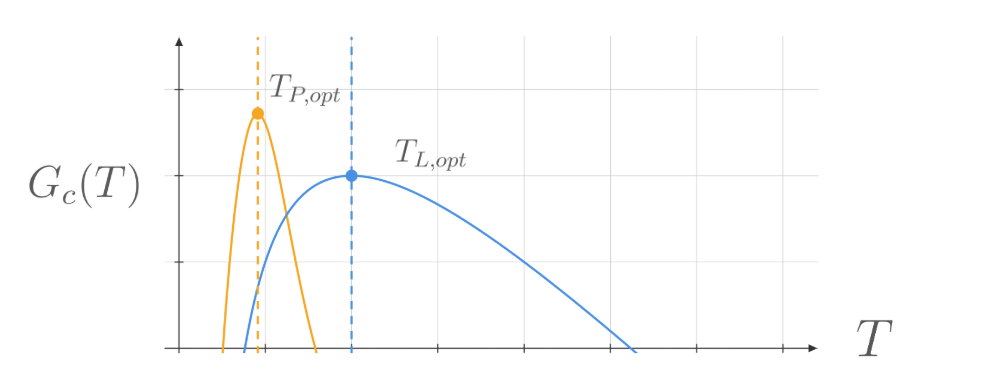
\includegraphics[width=0.95\textwidth]{figures/pred.png} 
    \caption{Optimal trait predictions under leaf economics (blue) and hydraulic-adjusted assimilation (orange) hypotheses. $G_c(T)$ is the assimilation rate as a function of a trait value $T$. $T_{P,opt}$ and $T_{L,opt}$ are the trait values where assimilation rate is maximized for the hydraulic-adjusted assimilation and leaf economics hypotheses respectively.}
    \label{fig:pred}
\end{figure} 

\section{Approach and Methods}

\subsection{Theory and modeling}
The first part of this chapter is a synthesis of trait-based models of single-leaf carbon assimilation with whole-plant growth and water use. Most of this initial phase has already been carried out, resulting in a simple framework that incorporates various leaf traits based on the general theory of leaf economics \cite{wang2023a, wang2017a, kikuzawa_cost-benefit_1991} along with allometric models of water use in trees \cite{kempes2011a}. The framework can be roughly separated into two distinct modules: (1) a biochemical model of single-leaf carbon assimilation and (2) allometric model of light interception, evapotranspiration, and water acquisition at the tree level. 

\subsubsection{Carbon assimilation}

At the leaf level, carbon assimilation is represented through a modified version of the model presented by Wang et al. \cite{wang2023a}, which is itself an extension of the Kikuzawa model \cite{kikuzawa_cost-benefit_1991}. Here, the instantaneous rate of carbon assimilation is represented as the sum of gross photosynthetic rate $A_{max}$, losses due to senescence ($B_{s}$), and construction costs ($C_c$).

\begin{equation}
    g(t) = A_{max}(1 - B_s(t)) - C_{c}(t)
\end{equation}

$A_{max}$ is the gross photosynthetic capacity, given average environmental conditions throughout the growing season. Senescence ($B_{s}$) is a time-dependent function and its progression follows a characteristic shape that is chiefly determined by LMA and the maximum rate of carboxylation \cite{xu_variations_2017}. 

\begin{equation}
    B_{s}(t) = \dfrac{t}{b}, \quad b = \dfrac{u LMA}{k_{1} k_{2} V_{cmax25}}
\end{equation}

Finally, $C_{c}$ is a time-varying function accounting for the carbon costs of constructing leaf tissues. The exact behavior of $C_{c}$ depends on leaf habit: deciduous trees make a single investment at the start of the growing season, whereas in evergreens construction costs accrue continuously. We estimate net carbon assimilation by averaging $g(t)$ throughout the year.

\begin{equation}
    \overline{g} =\dfrac{1}{365} \int_{s_{i}}^{s_{f}} A_{max}\left[1 - B_s(t)\right] - C_{c}(t) dt
\end{equation}

\subsubsection{Allometric scaling and hydraulics}

 Up to this point, carbon assimilation has been considered solely as a leaf-level phenomenon. Hereafter, we depart from previous analyses by integrating net assimilation across the canopy and incorporating whole-tree metabolism within the carbon budget. Canopy-wide carbon assimilation is treated further down, whereas losses due to metabolism are subtracted directly.

 \begin{equation}
    \overline{g} =\dfrac{1}{365} \left\{ A_{can}s_L\left[ 1 - \dfrac{s_L}{2b} \right] - \overline{C}_c\left(s_L, LMA, LL \right) - \beta_0 M^{\eta_0} \right\}
    \label{eq:net_g}
\end{equation}

Here, metabolism scales according to total tree biomass ($\beta_0M^{\eta_0}$) and annually averaged leaf construction costs are a function of growing season length $(s_L = s_f - s_i)$, LMA, and leaf longevity. In the case of deciduous trees, $\overline{C}_c$ is a single investment and is crucially determined by tree size, independent of either LL or LMA. The invariance of $\overline{C}_c$ with respect to LL and LMA in deciduous trees can be justified by noting that leaf longevity is constrained by $s_L$ and, given that photosynthetic biomass is necessarily proportional to total biomass \cite{niklas_invariant_2001}, LMA simply dictates how this biomass is allocated to leaf surface area.

To capture the relationship between leaf traits and climate, it is necessary to consider the effects of the environment on carbon assimilation as well as whole-tree water use. This, of course, requires a representation of canopy-wide energy budgets and light interception, as well as how the root system interfaces with soil moisture. This suite of processes is modeled after Kempes et al., \cite{kempes2011a}, including a few modifications which allow the integration of leaf traits, LMA in particular. Finally, the mathematical treatment of the biochemistry and physiology of photosynthesis is taken from the P-model \cite{stocker_p-model_2020}.

Having calculated the tree-wide rate of carbon assimilation and evapotranspiration, they can now be applied to equation \ref{eq:net_g}. The gross assimilation rate is substituted in $A_{can}$ directly, and the available flow rate of water ($Q_p$) is used to correct for potential water limitation. Water limitation is represented as a function of stomatal conductance $p(g_{ua})$, which is defined given a critical threshold $g_{crit}$:

\begin{equation}
    p(g_{ua}) = 
    \begin{cases}
         1 & \text{if $g_{ua} < g_{crit}$ }\\
         g_{ua}\omega/(g_{ua}g_{ul} - g_{ul}) & \text{otherwise}
    \end{cases}
\end{equation}

Here, $\omega$ subsumes the relationship between available evapotranspiration and the canopy's energy budget. As such, it is dependent on a suite of different functional traits, tree size, and climate. Further details of the model are omitted for brevity and are left for discussion elsewhere.


%paragraph on allometric model details (keep short, only essential details)


% Paragraph (and figures) presenting and interpreting preliminary results
Early simulations have shown that the model agrees qualitatively with the general trends leaf mass per area displays with climate variables, particularly with precipitation and temperature.

\begin{figure}[h!]
    \centering
    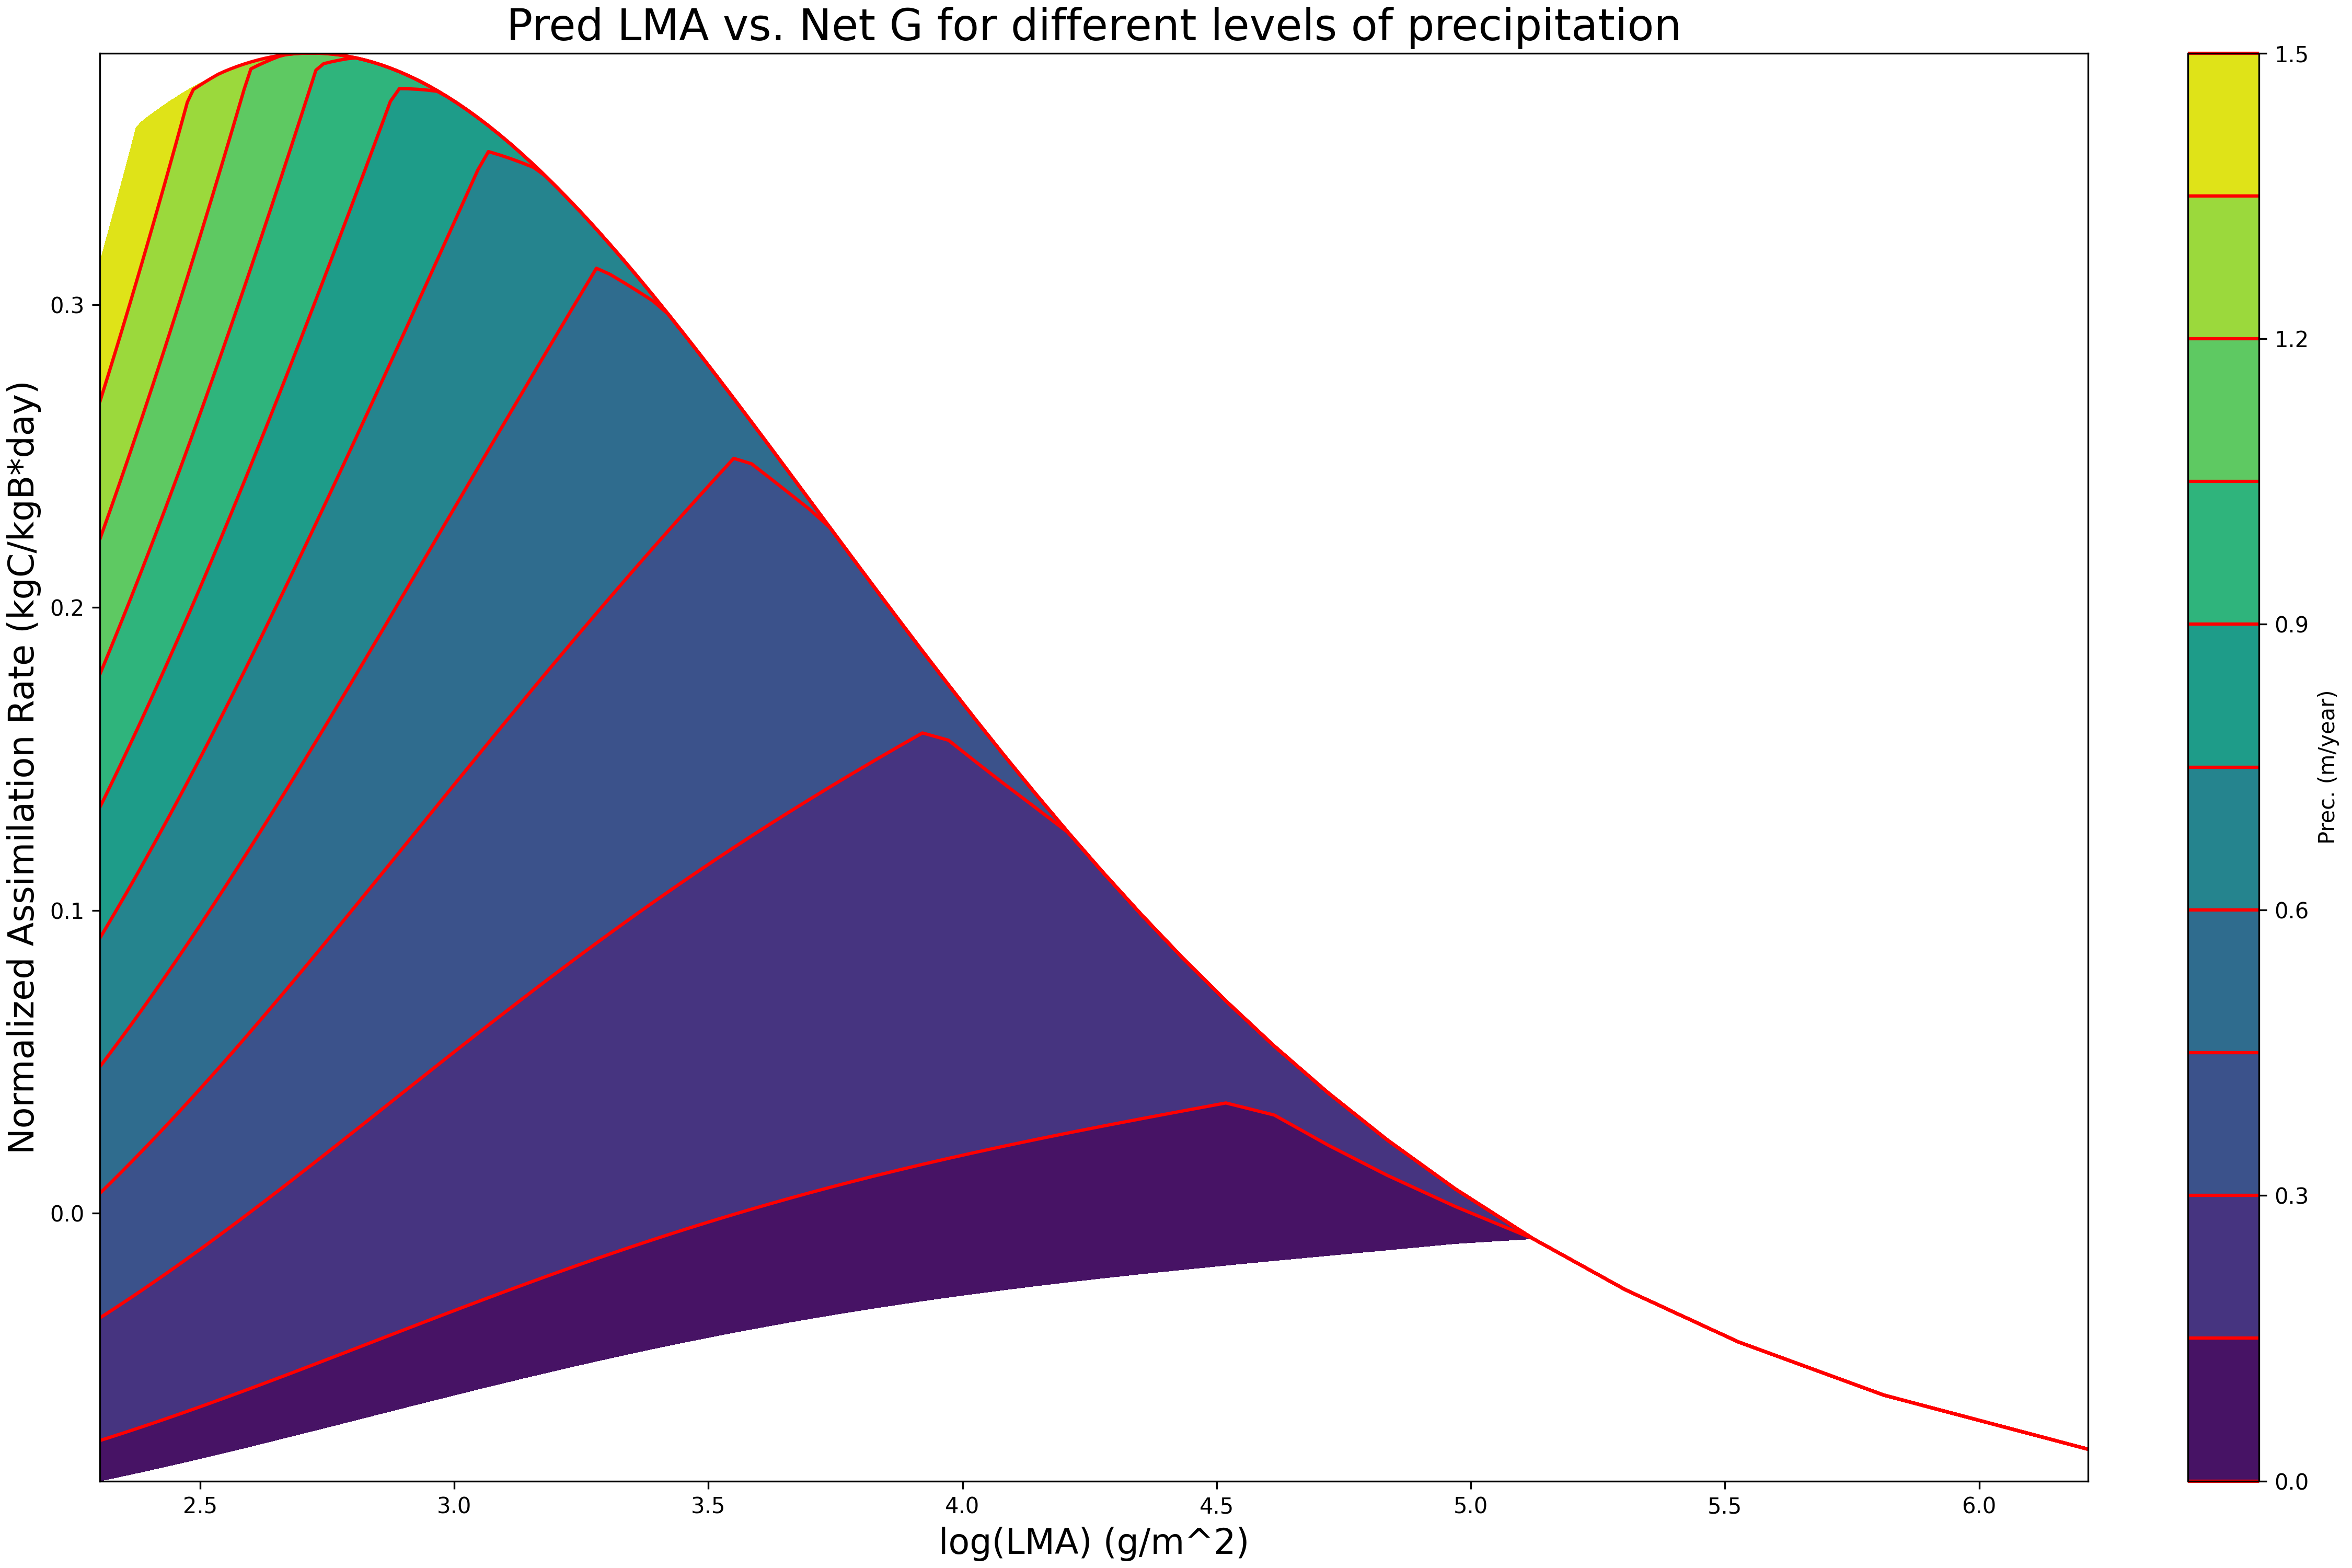
\includegraphics[width=0.95\textwidth]{figures/SLA_G_Pinc.png} 
    \caption{Normalized assimilation rate as a function of LMA and growing season precipitation. The simulations clearly show that the LMA at which assimilation rate is maximized shifts towards higher values as precipitation decreases which is consistent with observed global trends.}
    \label{fig:SLA_G_Pinc}
\end{figure} 

\subsection{Data and parameterization}
 
In order to make predictions it is necessary to parameterize and validate the model with empirical data. Fortunately, the model only has one free parameter, as all others are constrained through allometries or known physiological trade-offs. Validation will be carried out using trait data (cite data sources) containing abundance-weighted leaf mass per area moments, as well as the corresponding GPS coordinates. With the coordinates I will obtain the relevant climate variables through the CHELSEA geoclimatic models, along with estimated maximum tree heights found in the GEDI LIDAR database. A portion of the data will be used to parameterize stand water use efficiency, and the rest will be used to validate the model. 


% paragraph iving a detailed aount of data (variables, parameters, sources, other stuff)






\chapter{ Entropy dissipation and free energy availability as drivers of microbial community assembly}

\section{Background}

Microbial communities carry out a plethora of biochemical reactions through a diverse array of pathways, many of which are central to global biogeochemical cycles \cite{falkowski_microbial_2008}. Though there is excellent research showing how these reactions relate to microbial metabolism and growth at the individual and population level \cite{tang2017a}, it remains unclear how these principles scale to shape microbial communities. Most research concerned with the assembly and dynamics of microbial communities has focused on general rules arising from idealized trophic interactions \cite{bosi_perspectives_2017, van_den_berg_ecological_2022}, yet they do little to elucidate the mechanisms from which they emerge. Sequencing and metabolomic technologies have made it feasible to characterize how these reactions are structured at various spatial and temporal scales, offering a bioenergetic perspective on community dynamics (for a review, see \cite{kreft_genes_2017}). Here, I propose a method to reconstruct the thermodynamic properties of microbial metabolic interactions from genomically inferred reaction networks. The aim of this method and the corresponding chapter is to explore how thermodynamic forces impinge on the organization of microbial communities. 

% A paragraph on mechanistic models of microbial community assembly (as in community flux analysis, flux balance analysis, etc.)

Metabolic reaction networks are one of the primary tools used to understand how microbial populations interact with their environment. These networks allow us to map the potential pathways through which microbes process externally sourced substrates and whether these are ultimately assimilated into biomass or excreted as metabolic byproducts. The core principle which makes this kind of analysis possible is the application of stoichiometry to constrain the net flux of substrates through a reaction network. Furthermore, knowledge of the thermodynamic properties of key metabolic reactions (e.g. affinities and free energy yields) can offer additional details about the favorability of the corresponding pathways in a given environment \cite{kleerebezem2010a}. This general framework, commonly termed metabolic flux analysis, has been remarkably successful in reproducing empirical observations for different kinds of microbial systems \textcolor{red}{citations}. Despite this versatility, the simple formulation of the theory, in conjunction with its open ended assumptions, makes its application to highly diverse communities a persistent challenge. 

% Another paragraph exploring the common assumptions made about how microbial communities organize. What are the principles, optimization of some target function, approximated kinetics, etc.

Metabolic flux analysis (MFA), in its numerous manifestations, is subject to a set of fundamental constraints \cite{kooijman1998a, kleerebezem2010a}. Once applied to the dynamical equations, these constraints allow us to formulate the solution in terms of a system of underdetermined equations. In order to find acceptable solutions to the equations, it is often assumed that the microbial system optimizes a target quantity. For example, flux balance analysis is commonly performed under the supposition that microbial metabolism maximizes the molar yield of the network; however, it is clear that this is by no means a general organizing principle \cite{schuster_is_2008}. As such, the effectiveness of MFA is strongly dependent on the presupposed teleology of the microbial system. 

% A word about the main challenges, underdetermination of flux balance frameworks, difficulties in estimating absolute biomasses and corresponding fluxes, environmental tipping points. Explain how your approach helps resolve these challenges.

Beyond the challenge of selecting adequate optimization targets, there are a number of additional limitations associated with the application of MFA in complex microbial communities. A notable instance is the difficulty of justifying the steady-state condition for a large collection of microbes, given how unlikely it is that all members simultaneously prioritize biomass assimilation \cite{harcombe_metabolic_2014}. Of course, the steady-state condition can be relaxed through additional approximations (for example, \cite{khandelwal_community_2013, manhart_growth_2018}), though often with accompanying trade-offs. Further obstacles lie in providing realistic bounds for reaction rates and accounting for the costs of substrate transport. 

% A paragraph on extremization principles and hypotheses

In this chapter, I am proposing an extension of MFA that explicitly includes information on the thermodynamic properties of metabolic pathways such that state variables (e.g. free energy production and entropy dissipation) can be introduced as optimization targets. In addition to this, I plan to integrate the MFA framework into a spatially explicit substrate transport model, which would allow estimation of ecosystem-scale substrate fluxes. Following the development of the model, I aim to test whether soil ecosystems are organized by thermodynamic extremization principles such as, for example: the Maximum Power Principle \cite{odum_times_1955} and the Maximum Entropy Production Principle \cite{martyushev_maximum_2006}. 

\subsection{Hypotheses and Predictions}

As mentioned above, one of the key assumptions of the proposed method (and of MFA in general), is that microbial systems self organize towards an optimal objective function. Throughout I will be comparing the effectiveness of three differet objective functions at predicting steady state substrate concentrations and fluxes, each obejctive functions therefore represents a hypothesis. Hence, the Maximum Power Principle (MPP) predicts that the system will maximize the flow of free energy through the system, the Maximum Entorpy Production Principle (MEPP) maximizes the rate of entropy dissipation, and the Balanced Growth Hypotheses (BG) states that the biomass yield of the microbial community will be optmimized. To my knowledge, neither MPP nor MEPP have been tested as viable optimization targets for microbial communities despite being prominent concepts within ecosystem ecology \cite{odum_times_1955,meysman_thermodynamic_2007, unrean_metabolic_2011, endres_entropy_2017}

\section{Approach and Methods}

\subsection{Model development}

There exist many methods to approximate microbial growth from genomically inferred metabolic pathways \cite{kreft_genes_2017}. From these approaches, it is possible to explicitly derive how metabolism acts from a thermodynamic perspective, particularly in relation to entropy dissipation and free energy availability \cite{kleerebezem2010a}. In this chapter, I will incorporate the thermodynamics of microbial metabolic pathways into a larger description of soil nutrient cycling, focusing on how key microbial functional groups are constrained by environmental conditions. My approach builds on the general formulation of metabolic flux analysis by employing network thermodynamics as an additional source of constraints and optimization targets. As in traditional flux balance analysis, the system is initially defined in terms of the mass-action principle.

\begin{equation}
    \Delta_{t} S_{\alpha} = (S_{\alpha}^{I} - S_{\alpha}^{O}) + \sum_{i} \sum_{k} q_{ki}\gamma_{\alpha k} - B_{i\alpha} 
    \label{eq:massact}
\end{equation}

Equation \ref{eq:massact} states that the change over time in the concentration of substrate $S_{\alpha}$ is given by the influx from an external pool ($S_{\alpha}^{I}$), conversion reactions carried out by microbes ($q_{ki}\gamma_{\alpha k}$), assimilation into microbial biomass ($B_{i\alpha}$), and outflow ($S_{\alpha}^{O}$). Stoichiometric coefficients ($\gamma_{\alpha k}$) are known from pathway biochemistry, while reaction rates ($q_{ki}$ and $B_{i\alpha}$) are determined by a subsequent optimization procedure. Inflow and outflow rates are governed by transport models, which will be discussed elsewhere.

In order to solve equation \ref{eq:massact}, we must either postulate a set of dynamical equations for each chemical reaction, or assume that the system can be approximated as a stationary process. In the latter case, we must introduce a version of the steady-state condition; for example, by setting eq. \ref{eq:massact} to zero.

\begin{equation}
    (S_{\alpha}^{I} - S_{\alpha}^{O}) + \sum_{i} \sum_{k} q_{ki}\gamma_{\alpha k} - B_{i\alpha} = 0
    \label{eq:MASS}
\end{equation}

This is the core assumption of flux balance analysis, which allows us to ascertain the structure of the community by means of an optimization problem. Since the system of equations defined by eq. \ref{eq:MASS} is of smaller order than the number of unknown quantities (typically $q{ki}$ and $B_{i\alpha}$), it is necessary to assume an \textit{a priori} optimization target to select among the infinite possible solutions. The search space of the problem can be reduced through the introduction of additional constraints. For instance, there are known biological or chemical limits for certain reactions, these can be used to bound the corresponding rates.

\begin{equation}
    q_{ki}^{min} \leq q_{ki} \leq q_{ki}^{max}
\end{equation}

We can move beyond traditional MFA by considering the thermodynamic properties of each metabolic pathway. Specifically, the Gibbs free energy yield of catabolic and anabolic reactions can be estimated from stoichiometric coefficients in addition to the Gibbs energy of formation of individual compounds. Whole-network thermodynamics can be further resolved through the use of known biomass yields. Given a single metabolic pathway, Gibbs free energy yield is given by:

\begin{equation}
        \Delta G_{Met} = \lambda_{Cat} \Delta G_{Cat} + \Delta G_{An} + \Delta G_{Dis} = 0
\end{equation}

$\Delta G_{Cat}$, $\Delta G_{An}$, and $\Delta G_{Dis}$ are the Gibbs free energies of catabolic and anabolic reactions plus the dissipated free energy. $\lambda_{Cat}$ represents the efficiency of biomass formation, that is, how many times the catabolic reaction needs to be carried out to yield one unit of biomass. Although there are important subtleties in the precise calculation of each of these terms, I delegate that discussion to the broader literature \cite{kleerebezem2010a, desmond-le_quemener_thermodynamic_2014}. Gibbs free energies can be used to estimate whole network state variables such as entropy production.

\begin{equation}
         \sigma_{Net} = \sum_{i} \dfrac{\Delta G^{Met}_{i\alpha}}{T} \dfrac{d\xi^{Met}_{B, i}}{dt} = \sum_{i \alpha} \dfrac{\Delta G^{Met}_{i\alpha} B_{i\alpha}}{T} 
     \end{equation}

Finally, network thermodynamics facilitate the construction of fundamental energetic constraints applicable to systems more generally (e.g. reversibility conditions for specific chemical reactions). 

%Furthermore, give some indication of how you plan to incorporate resource transport mechanisms.

Before applying the MFA model presented above to soil ecosystems, it must be coupled to a spatially explicit transport model so that substrate concentrations are able to diffuse along the soil column. This will be accompished by modifying the DETECT model \cite{ryan_modeling_2018} so that substrate production rates are governed by the flux balances obstained from MFA. Likewise, substrate inflow and outflow will be constrained via DETECT's dtransport mechanisms. 

\subsection{Empirical validation}

% We don't currently have a plan for empirical validation, but we can give a rough idea of how this might be done using EMERGE data. Maybe point out the plethora of genomic data and the possibility of using corresponding flux measurements and metabolomic data.

% focus rather on specifying a pipeline, as in the Hough paper.

% A few sentences on coarse grained observables, such as soil NOSC and biomass estimates using chloroform fumigation.

Having defined the modeling formalism, is is necessary to propose an empirical scheme within which the hypotheses and corresponding predictions can be compared. First, I will summarize the data pipeline which will be used to parameterize the MFA and underlying constraints. This includes the reconstruction of microbial metabolic networks using metagenome assembled genomes (MAGs), initializing constraints and transport model with available soil chemistry and plant productivity data, and integration of substrate thermodynamics into network analysis. Lastly, I give a sketch of how model predictions will be compared and tested with a combinaiton of metabolomics, chamber gas fluxes, and metatranscriptomics.

\subsection{Modeling Pipeline}

The coupled MFA and substrate transport model require 4 main types of data: (1) presence/absence of metabolic pathways to reconstruct microbial networks, (2) initial substrate input rates estimated from plant litter decomposition, (3) physico-chemical properties of the soil matrix at different depths (e.g. temperature and pH), and (4) thermochemical data for the range of available substrates. The first three types of data will be sourced from the EMERGE BII database, which contains over 10 years data from the long-term investigation of the permafrost system in Stordalen Mire, Sweden. Metabolic pathway infromation will be inferred from MAGs sequenced from soil cores at different depths, and annotated using microTrait \cite{karaoz2022a}. Substrate input rates will be esitmated from previous measurements of litter decomposition rate for different types of vegetation \cite{hough2022a}. Soil physico-chemistry will be taken from EMERGE biogeochemistry datasets. Lastly, thermochemical data will be pulled from the NIST reference database \cite{p_nist_1998}.

\subsection{Model Comparison and Hypothesis Testing}







\chapter{Linking ecosystem size distributions to environmental disturbance regimes}

\section{Introduction and Justification}

Forests are fundamental to Earth's biosphere, regulating carbon, energy, and water cycles at planetary scales. They store over $40\%$ of terrestrial carbon and drive more than half of the net primary productivity \cite{bonan_forests_2008, pan_large_2011}. Terrestrial vegetation makes up the majority of biomass on earth, fueling virtually every biochemical process in the biosphere \cite{bar-on_biomass_2018}. Despite their ecological and societal importance, forests remain a significant source of uncertainty in climate projections. This is mainly due to the paucity of large-scale data capable of constraining carbon turnover rates and predicting responses to disturbance \cite{doughty_tropical_2023, friedlingstein_global_2023, pugh_understanding_2020}. To improve climate models, we must develop scalable, predictive approaches for assessing forest resilience and disturbance.

Due to their ecological and societal value, forests have a long history of meticulous monitoring; ranging from long-term field studies to national inventories. Forest monitoring has evolved from field-based inventories to sophisticated remote sensing approaches, promising global coverage with increasing temporal and spatial resolution. These efforts have provided critical data for carbon budgeting and revealed patterns in forest structure, biogeography, and demographics \cite{duncanson_assessing_2015,friedlingstein_global_2023}. In addition, remote sensing is widely adopted into inventory and monitoring strategies, promising unprecedented spatial coverage and temporal resolution \cite{fassnacht_remote_2024, duncanson_aboveground_2022}. However, despite these advances, precise quantification of disturbance remains challenging (Gao et al., 2020). Current vegetation models often rely on historical correlations, but nonlinear feedbacks between forest biota and the Earth system likely introduce tipping points that undermine conventional projections \cite{dietz_economic_2021, lenton_environmental_2013}. There is a pressing need for scalable and reproducible methods that link large-scale tree dynamics to underlying environmental processes, including anthropogenic change. 

A key concern in existing vegetation dynamic models is the reliance on historical correlations of net carbon assimilation with numerous biotic and abiotic factors \cite{allen_underestimation_2015, barnes2022a}. For example, the Amazon rainforest’s response to severe drought events has been shown to vary considerably \cite{anderegg_divergent_2020, saleska_amazon_2007}. Recent work has demonstrated that incorporating information about local environmental conditions (e.g. topography and water table depth), as well as focal functional traits, explains a significant portion of the residual variation \cite{chen_amazon_2024, signori-muller_non-structural_2021, tavares_basin-wide_2023}. However, in most instances it is a priori unknown which biotic and abiotic factors will be important, making it difficult to generalize across forest ecosystems. 

Anticipating the effects of particular stressors on tree communities is particularly challenging due to the numerous feedbacks. Ecosystem responses to novel environmental regimes largely depend on their historic exposure to different disturbance types and existing functional variation \cite{renes_disturbance_2020, hoffmann_environmental_2000}. A corollary of this is that not all species will react proportionally to the same conditions. Thus, community resilience can only be fully quantified through large-scale trends in species abundance distributions \cite{loreau2010a, arnoldi_how_2018}. Distribution patterns have been used to identify susceptible ecosystems in numerous studies \cite{chaalali_species_2016, padfield_linking_2018, pecl_biodiversity_2017} and have proven to be especially insightful when paired with process-based modeling \cite{dakos2011a}. 

Forests across the globe display an astonishing diversity of functional traits, many of which are closely related to environmental conditions \cite{lopez_coordination_2021, reich2014a}. A few traits vary so consistently across large climatic and taxonomic ranges to indicate the dominance of highly conserved physiological constraints \cite{delong_shifts_2010, hatton2019a, wright2004a}. Among these, body size (i.e. tree height) is perhaps the most well-established due to its close association with organismal metabolic rate, as well as its implications for ecosystem-wide energy fluxes \cite{allen2005a, brown2004a, savage_sizing_2008}. Beyond its relationship with energetic expenditure, the importance of tree size is made apparent through robust structural and functional allometries \cite{chave_improved_2014, goodman_importance_2014, niklas_invariant_2001}. Indeed, numerous studies have leveraged size-abundance distributions to assess the general health and functionality of various biological systems \cite{chaalali_species_2016, guo_size_2022, spanbauer_body_2016}. However, despite the widespread use of allometric scaling in estimating aboveground carbon sequestration, its implications for forest resilience and robustness remain largely unexplored. 

Interpreting size-abundance distributions is facilitated when framed within theoretical models of size-structured vegetation growth. These models divide trees into size classes and assume that growth is given by a combination of resource acquisition, basal metabolism, mortality, and competition. A general formulation is given by the Von Foerster equation, where the change in abundance of size class, defined as all trees of height $h$, ($h_{k-1} \leq h \leq h_{k} $), is given by the growth of smaller size classes ($N_{k-1}$) at rate $\dot{h}_{k-1}$, minus growth into larger trees ($\dot{h}_{k}$), minus a mortality term, $\mu_{k}$. 

\begin{equation}
    \dfrac{dN_{k}}{dt} = \dfrac{N_{k-1}\dot{h}_{k-1}(R) - N_{k}\dot{h}_{k}(R)}{h_{k}-h_{k-1} }  - \mu_{k}N_{k}
\end{equation}

In principle size classes can be made arbitrarily small, rendering a system of partial differential equations. Detailed analyses of such continuous size models have been previously carried out \cite{enquist_scaling_2024, lee_growth_2021, moorcroft_method_2001,  odwyer_integrative_2009}, yielding expected equilibrium size distributions and subsequent deviations caused by different forms of perturbation. If we part from the most basic set of assumptions, that is, that growth and mortality scale as power functions of height ($g(h) = ah^{c} $ and $m(h)=rh^{b} $ ) the resulting, normalized steady state distribution (henceforth SSD) is given by a Weibull distribution \cite{muller-landau_comparing_2006}.

\begin{equation}
    P(h) = \dfrac{1}{N_{0}} h^{-c} \exp{\left[ \dfrac{-ah^{1+b-c}}{r(1 + b -c )} \right]} 
\end{equation}

The generality of size-structured frameworks has lent itself to a wide range of applications; in particular its adoption in Earth System Models (ESM) such as the DOE’s ELM-FATES which is derived from the Ecosystem Demography Model \cite{fisher_taking_2015, moorcroft_method_2001}. ESMs have likewise been used to simulate and inform understanding of forest disturbance dynamics \cite{shi_functionally_2024}. Though the granularity of complex models such as FATES is indispensable to generate fine-scale predictions, there is a need for coarse-grained approaches that allow us to assess general patterns of ecosystem structure, and identify large-scale signatures of disturbance. 

\section{Approach and Methods}

Here, I propose a novel approach for quantifying forest robustness and resilience based on allometric models of vegetation growth and size-abundance distributions inferred from remote sensing. This research consists of three components: (1) Mapping global forest height distributions using GEDI LiDAR waveforms and SAR tomography. (2) Using size-abundance distributions and climate data to parameterize size-structured vegetation models and establish baseline expectations. (3) Comparing modeled predictions to forests with known disturbance regimes (i.e. managed forests) to generate quantitative disturbance profiles. 

\subsection{Mapping global forest height distributions with remote sensing}

Advancements in remote sensing now allow for the reconstruction of forest structure with increasing accuracy. In particular, GEDI LiDAR has proven to be especially valuable for above-ground biomass estimation, especially when paired with other remote sensing tools and calibrated with field data \cite{chi_national_2015, crockett_structural_2023, potapov_mapping_2021}. Although uncertainties exist in tree height estimation, recent studies indicate that GEDI can accurately capture normalized height frequency distributions which better reflects size structure \cite{tan_exploring_2024}. Specifically, Ngo et al., \cite{ngo_tropical_2022} demonstrated that GEDI waveforms accurately characterized the vertical structure of tropical forests when combined with P-band synthetic aperture radar (SAR) tomography (Figure 2).

I will use forest inventory data to calibrate a pipeline that infers height frequency distributions from GEDI waveforms in conjunction with existing SAR tomography datasets, such as TanDEM-X, TerraSAR-X and ESA’s upcoming BIOMASS mission. We will borrow from recently developed remote sensing methods and leverage existing models that estimate size structure from field-based measurements \cite{ngo_tropical_2022, ramachandran_evaluation_2021}. 
The first stage of the pipeline will identify appropriate datasets with which to train and validate the inference procedure. The selection process will be based on criteria laid out by Crockett et al. \cite{crockett_structural_2023}, emphasizing the requirement that forest plots be sampled from 2017 and that they be at least 90\% forested. Currently this includes at least 1796 FIA plots and will likely extend to similar inventory data so long as it contains diameter at breast height (DBH) measurements. DBH measurements will be used to predict stand-level diameter distributions using a Maximum Entropy model described in \cite{chen_stand_2019}.

Field-based diameter distributions will then be used to train and evaluate models that predict size-abundance distributions from GEDI waveforms and SAR backscatter profiles. Two main modeling approaches will be compared: deep learning with convolutional neural networks based on the FORMS model \cite{schwartz_forms_2023}, and random forest regression coupled with Monte Carlo simulation \cite{li_aboveground_2022}. Both of these approaches have shown promising results in estimating above ground biomass from remote sensing data, and we expect similar performance when estimating size distributions.

\subsection{Baseline Predictions in Pristine Forests}

This portion of the chapter will use data from pristine forests to parameterize a general model of vegetation growth. The purpose of this is to provide threshold expectations for how climate and biogeography impact forest height structure in the absence of long-term perturbations. Environmental parameters will be constrained through historical average precipitation and photon flux densities derived from climate models. I present a slightly modified version of the Von Foerster model to explicitly incorporate stochasticity.

\begin{figure}[ht!]
    \centering
    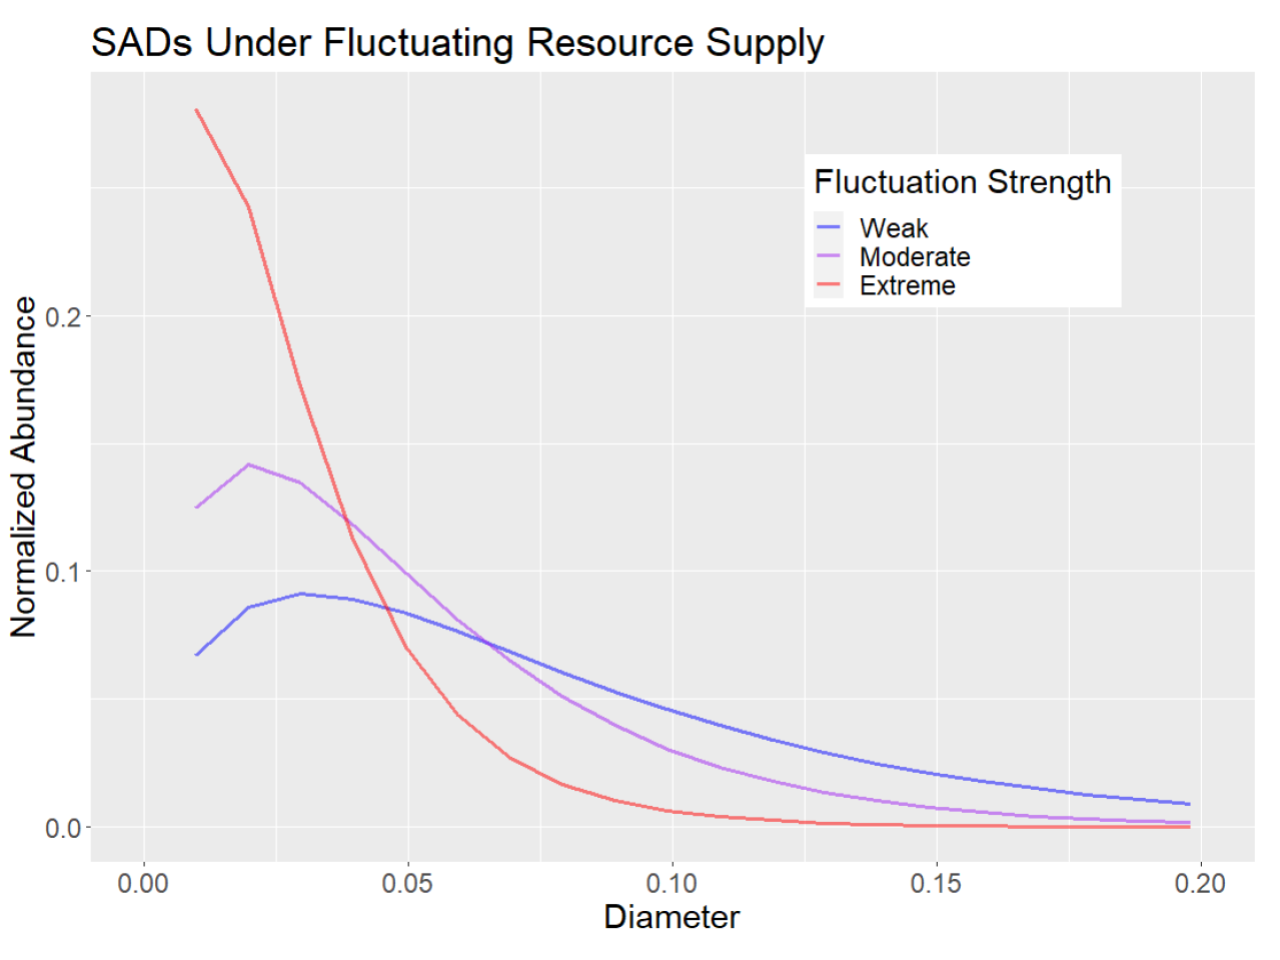
\includegraphics[width=0.8\textwidth]{figures/SAD_fig.png} 
    \caption{Size-abundance distributions from an early implementation of the size-strucutured model. This proof of principle illustrates how resource fluctuations shape the SAD under different resource fluctuation regimes. The distribution shifts towards smaller trees as fluctuations become more severe.}
    \label{fig:SAD}
\end{figure} 

\begin{equation}
    \dfrac{\partial N(h, t)}{\partial t} = \dfrac{\partial}{\partial h} [N(h, t)\dot{h}(h)] - N(h, t)\left[\mu(h, t) + \int_{h_{0}}^{\infty}\alpha(h, h^{\prime})N(h^{\prime}, t)dh^{\prime} \right]
\end{equation}

The first term on the right-hand side describes the average growth of the size distribution in ideal, resource-replete conditions. The following term quantifies how environmental conditions and biotic interactions impact forest-wide variation in growth rates. Hence, assuming that fluctuations in mortality and resource supply follow a given functional form, the SSD can be related to the prevalence of disturbance and competitive interactions. Furthermore, assessing the system’s susceptibility to acute and chronic perturbations can be straightforward through analytical and numerical means (Figure 3). Mortality, $\mu(h, t)$, can be represented as a stochastic process.

\begin{equation}
     \mu(h, t) = \mu_{W}(h)dW
\end{equation}

The size dependence of $\mu_{W}(h)$ considers that disturbance events may preferentially impact trees of a particular height. The effect of fluctuating resources can be incorporated as a modification to the basal growth rate which accounts for resource limitation.
\begin{equation}
    \dot{h}(t, h) =g_{0}h^{c} \dfrac{V(h)\rho(t)}{V(h)\rho(t) + Q_{0}(h)K(h)} - \mu_{o}h^{b} ,  \quad K(h) =\dfrac{g_{0}h^{c}}{\mu_{0}h^{b}} - 1 
\end{equation}

Here $V(h)$ represents a harvesting volume and $Q_{0}(h)$ is the basal metabolic demand for a tree of a given size. Assuming that $V(h)$ is proportional to the radial extent of the root system and $Q_{0}(h)$ is set by maintenance metabolism,  harvesting volume and basal demand can be defined as power functions of $h$ as per \cite{kempes2011a, niklas_growth_2004}. Additionally, $\rho(t)$ is the time-fluctuating density of resources with mean $\rho_{0}$.

The time dependence denoted by $\chi(t)$ can be modeled as colored noise based on observed supply time-series, such as the one provided by the standardized precipitation evapotranspiration index (SPEI) \cite{begueria_standardized_2014}. Finally, we assume that competition is inversely proportional to an exponent of height, requiring that competitive burden decrease as trees get taller.

\begin{equation}
    \beta_{0}h^{-\alpha} \sim \int_{h_{0}}^{\infty} \alpha(h, h^{\prime})N(h^{\prime})dh^{\prime}, \quad \rho(t) = \dfrac{\rho_{0}}{\chi(t)}
\end{equation}


Having defined the system in this manner and assuming that intact forests are dominated by resource supply and metabolic demand constrains nearly all parameters through robust allometric relationships and climate. Hence, the fitting procedure is only concerns the interaction structure of the underlying vegetation ($\beta_{0}h^{-\alpha}$).

\subsection{Characterizing Disturbance From Deviations in Managed Forests}

Using results from Task 2, I will analyze forests with biogeographic adjacency but varying disturbance regimes. The premise is that forests with similar interaction structure and climate should exhibit comparable size-abundance distributions in the absence of disturbance. By comparing disturbed forests to baseline expectations, I will quantify the impact of different disturbance types. This involves (1) Identifying forests with independently quantifiable, above baseline mortality rates; and (2) using inferred height profiles to parameterize added mortality.



    
\chapter{Metabolomic imprint of plant life history strategies}


Idea: Many plant functional traits are tightly correlated with specific life history strategies which impact how plants grow and reproduce. Some of these traits concern the stoichiometry and composition of different plant tissues (e.g. carbon:nitrogen and carbon:phosphorus ratios), showing some promising trends. In this chapter I am proposing to look a little bit closer at the chemistry of plant tissues, try and parse out what they are composed of, how many carbons, hydrogens, nitrogens, aromatic rings, etc. Ultimately, I want to see if there is a relationship between the lability/recalcitrance of plant tissues/exudates and their particular life history strategies.
Question: Do plant life history strategies dictate the free energy availability of plant litter and root exudates?

\section{Background}

%First paragraph introducing the problem: how can we tie above ground productivity to below ground carbon dynamics? How do plant communities impact microbial life in their immediate suroundings, and vice versa? Hint at plant functional traits and the leaf economics spectrum as a potential theoretical link. 

Carbon and nutrient cycling in terrestrial ecosystems is predominantly driven by intricate relationships between above-ground primary producers and soil microorganisms. These relationships, though strongly mediated by soil properties and local abiotic factors, airse through a series of biochemical transformations ranging from photosynthesis in plants to numerous metabolic reactions carried out by microbes. If we consider that plants and their corresponding soil inputs are the predominant source of organic carbon in terrestrial ecosystems, it follows that the range of fesible metabolic activities is generally constrained by the quantity and quality of plant derived organic matter. Furthermore, given the systematic covariation between environmental conditions, plant functional types, and plant litter composition \textcolor{red}{citations}; we should observe consistent relationships linking above ground plant communities to below ground microbial decomposition. Although there is evidence to support the existence of these relationships \textcolor{red}{citations}, our understanding remains largely descriptive and lacks a consistent framework grounded in plant energetics and biochemistry. Here I explore a new method of framing the biochemical ramifications of plant functional traits and life history theory with the aim of refining our predictions for soil carbon and nutrient cycling. 

% Second paragraph going into detail on the stoichiometric implications of the LES and life history theory, name a few of the main hypoetheses in this sphere, cite relevant papers.

As mentioned in prior chapters, plant life history strategies have important implications for numerous features of plant form and function, not least of which is the stoichiometry of various plant tissues \cite{reich2014a,wright2004a}. Hence, the chemical composition of plant derived organic matter can be tied to the preponderance of plant functional types via economic and energetic principles. For example, the LES predicts that faster growing species will have a higher mass-normalized leaf content of Nitrogen and Phosphorous relative to slower growing species, mainly due to the high N and P concentrations of metabolically active proteins \cite{diaz_global_2016}. Meanwhile the foliar ratio of N:P should show a negative correlation with maximal relative growth rate, which is attributed to the elevated demand for protein synthesis and the corresponding enrichment in ribosomal RNA, ribosomal DNA, and the length increase of intergenic spacer regions \cite{gusewell_n_2004, elser_biological_2000}. Despite the consistency between observed trends in plant stoichiometry and the cellular mechanisms proposed to explain them , the precise drivers remain difficult to identify given the large degree of inter- and intraspecific variation, as well as confounding effects arising from ecological interactions (e.g. herbivory and soil nutrient content).

% Third paragraph intoduces the how the LES and life history theory could have deeper ramifications regarding soil microbial activity. Again, introduce some of the well known ideas and cite important papers.

Now, turning to the impact of plant chemical composition on downstream microbial activity, it is quite clear that elemental ratios reflect the preponderance of key limiting processes, such as the link between C:N ratios and decomposability \cite{bakker_leaf_2011}. For example, Manzoni et al. found that low carbon:nutriet ratios (C:N and C:P) effectively reduce the carbon use efficiency of decomposers \cite{manzoni_stoichiometric_2010}. However, nutrient contents -- in terms of coarse grained elemental ratios -- do not always accurately predict the subsequent carbon dynamics due to potential constraints affecting bioavailability, such as the environmental concentration of terminal electron acceptors (TEAs). In scenarios where substrate decomposition is strongly modulated by TEA availability (e.g. wetlands) it is more infromative to consider measures of thermodynamic favorability as these directly relate to the energetic yield of substrates upon oxidation \cite{kleerebezem2010a,hough2022a}. In light of this, we might wonder: how do plant functional types relate to the thermodynamic favorability of the corresponding litter?

% Final paragraph of intro, give a rough idea of how the relationship between plant litter stoichiometry and functional traits can be expanded upon to infer further details on the decomposability of above ground carbon inputs. Elaborate on how metabolomic metrics such as NOSC can be used to improve our predictions of the linkage between plant and soil communities.

This final chapter explores how plant form and function--that is, where functional traits fall on the spectrum of life history strategies--impacts the thermodynamic favorability of plant derived carbon inputs as inferred from the corresponding metabolomic signature. Initially, this will imply extending the theory of leaf economics to include predictions for how key metabolite concentrations (namely, structural polymers and primary metabolites) relate to the different axes of the LES. Successively, I aim to use predicted metabolite balances to justify a theoretical link between life history strategies and the thermodynamic favorability of photosynthetic tissues. After consolidating a theoretical backbone, I will test the resulting predictions against empirical measurements; comparing leaf leaf litter metabolomes, energetic favorability metrics such as the nominal oxidation state of carbon (NOSC), and decomposition dynamics under variable conditions. 

\section{Approach and Methods}

% First paragraph is a summary of the overall approach. Firs elaborate on the extent of the theory, how will you modify current theory to include energetic measures such as NOSC. Next, mention that you will use metabolomics and EMERGE data to test these ideas. Summarize, in a succinct sentence, state what this work will accomplish.

As this chapter is the least developed in my proposed dissertation, I will refrain from presenting the approach in detail. For the present moment I will give an overview of the steps needed to develop a satisfactory theoretical and empirical link between plant life history and the energetic favorability of photosynthetic tissues. As for the theory I will leverage biochemical models of photosynthesis and, in concordance with the LES, relate the magnitude of key functional traits to the relative abundance of metabolically active compounts in photosynthetic tissues. With a putative mechanism driving metabolite balances, it will then be possible to infer how the NOSC leaf litter varies as a function of plant life history. The empirical portion of the chapter will consist of drawing comparisons between prior theoretical predictions and field based measurements of leaf metabolomics, NOSC, and decomposition rates in incubation experiments.

% subsection: Elaborate theory of PFT and litter bioavailability   

\subsection{Theory}

The chemical composition of plant photosynthetic tissues is broadly composed of structural polymers, primary metabolites involved in core physiological processes, non-structural carbohydrates, lipids, proteins, and a diverse array of secondary metabolites. Each of these categories corresponds to a defined set of functional roles and, to a certain extent, have well conserved metabolomic profiles. For example structural polymers, the content of which is strongly tied to specific fucntional traits (e.g. leaf dry matter content and SLA), are largely comprised of cellulose, hemicellulose, and lignins. Therefore higher abundance of structural polymers should correlate negatively with nutrient content and energetic favorability. Similarly, maximum photosynthetic capacity is directly linked to the concentration of metabolically active proteins and enzymes thus, by using biochemical models of leaf metabolism it is possible to make quantitative predictions for how photosynthetic capacity relates to the concentration of primary metabolites \cite{vipina_modelling_2025, paul_carbon_2003}. 

Other compounds play variable roles in plant life history and cannot be assigned specific functions with as much confidence, nonetheless they present an interesting opportunity for exploring additional facets of plant functional traits. As an example, it would be interesting to investigate how secondary metabolite content varies in response to herbivory, or how lipid content relates to succulence as measured by leaf water content. Another thread worth interrogating is how leaf lifespan relates to the presence of antimicrobial metabolites, such as the presence of polyphenols, terpenes, and alkaloids. Though not a precisely defined, life history theory and the LES can enable qualitative predictions for how these compounds covary with respect to global spectrum of plant form and function.

% subsection: Propose method of testing predicitons with EMERGE (or other) datasets
 \subsection{Empirical}

 To test the predictions resulting from the theoretical portion of this chapter it will be necessary to compare to data which simultaneously relates the presence of functional traits with respect to leaf metabolomics and, when available, decomposition dynamics. As a tentative dataset, I am proposing a comparison with the results of Hough et al., which detail the relationships between plant functional type, leaf litter metabolomics, energetic favorability (as measured by NOSC), and decomposition rates across a permafrost gradient \cite{hough2022a}. However, as this dataset is lacking several of the central LES functional traits, it will likely be necessary to either supplement it with trait data from Stordalen Mire, or extrapolate from similar species in different sites.

%%%%%%%%%%%%%%%%
% References
%%%%%%%%%%%%%%%%
\begin{singlespace}  % use single-line spacing for multi-line text within a single reference
\setlength\bibitemsep{\baselineskip}  %manually set separataion betwen items in bibliography to double space
\printbibliography[title={References}]
\end{singlespace}

\addcontentsline{toc}{chapter}{References}  %add References section to Table of Contents

%%%%%%%%%%%%%%%%
% Appendices if applicable
%%%%%%%%%%%%%%%%
% Use package `appendix`
% \begin{appendices}

%Some Table of Contents entry formatting
\addtocontents{toc}{\protect\renewcommand{\protect\cftchappresnum}{\appendixname\space}}
\addtocontents{toc}{\protect\renewcommand{\protect\cftchapnumwidth}{6em}}

%Begin individual appendices, separated as chapters

\chapter{Experimental Equipment}
Lorem ipsum dolor sit amet, consectetur adipiscing elit, sed do eiusmod tempor incididunt ut labore et dolore magna aliqua. Ut enim ad minim veniam, quis nostrud exercitation ullamco laboris nisi ut aliquip ex ea commodo consequat. Duis aute irure dolor in reprehenderit in voluptate velit esse cillum dolore eu fugiat nulla pariatur. Excepteur sint occaecat cupidatat non proident, sunt in culpa qui officia deserunt mollit anim id est laborum.

\chapter{Data Processing}
Lorem ipsum dolor sit amet, consectetur adipiscing elit, sed do eiusmod tempor incididunt ut labore et dolore magna aliqua. Ut enim ad minim veniam, quis nostrud exercitation ullamco laboris nisi ut aliquip ex ea commodo consequat. Duis aute irure dolor in reprehenderit in voluptate velit esse cillum dolore eu fugiat nulla pariatur. Excepteur sint occaecat cupidatat non proident, sunt in culpa qui officia deserunt mollit anim id est laborum.

\end{appendices}

\end{document}
